\chapter{Ensemble learning: forests, boosting, and model combination}
\label{ch:ensembles}

\begin{learningobjectives}
After this chapter, you should be able to:
\begin{itemize}
  \item distinguish bagging, random forests, extra trees, boosting, voting, and
  stacking by the mechanism that creates and combines learners;
  \item derive the variance of an average under correlated member errors and
  explain why diversity matters;
  \item derive squared-error gradient boosting as stagewise residual fitting;
  \item construct out-of-fold features for leakage-safe stacking;
  \item evaluate discrimination, probability quality, stability,
  interpretation, and resource cost; and
  \item design reusable ensemble code, behavior tests, and a defensible
  champion--challenger promotion gate.
\end{itemize}
\end{learningobjectives}

\begin{chapterconnection}
A decision tree learns nonlinear interactions and an interpretable partition,
but small changes in its training observations can produce different early
splits and a different tree. Ensemble learning turns variation among fitted
learners into a design variable. Bagging and random forests average perturbed
learners to reduce variance. Boosting constructs a sequence of corrections to
reduce loss. Voting and stacking combine heterogeneous inductive biases. These
mechanisms share multiple members, but not the same mathematics, data flow, or
failure modes.
\end{chapterconnection}

\section{The organizing question: where does useful diversity come from?}

An ensemble produces a prediction from member functions
$F_1,\dots,F_M$. Its benefit cannot follow from member count alone. If every
member makes the same error, repeating it changes nothing. If members are
independent but useless, their average remains useless. A successful ensemble
requires two properties:
\begin{enumerate}
  \item \emph{competence}: members carry information about the target; and
  \item \emph{diversity}: members do not reproduce exactly the same error.
\end{enumerate}

Different methods create diversity differently. Bagging perturbs observations.
Random forests perturb observations and candidate features. Extra trees also
randomize thresholds. Boosting changes the pseudo-response or example weights
at every stage. Voting and stacking combine model families with different
representations. Evaluation must identify which mechanism is being used rather
than calling all of them ``many models.''

Historically, ensemble learning joins ideas from statistics, computational
learning theory, and numerical optimization. Breiman introduced bootstrap
aggregating, or \emph{bagging}, in 1996 and random forests in 2001. Ho developed
random-subspace methods in the 1990s. Schapire showed that weak learnability can
imply strong learnability; Freund and Schapire's AdaBoost made sequential
reweighting practical. Friedman later formulated gradient boosting as
optimization over functions. Wolpert's stacked generalization combines
heterogeneous models using a learned second level. The chronology matters
because these algorithms solve different problems, not because newer always
means better.

\section{Why averaging can reduce variance}

Let $E_m=F_m(X)-Y$ denote member $m$'s prediction error. Suppose, as a
simplifying model, that
\[
  \operatorname{Var}(E_m)=\sigma^2,
  \qquad
  \operatorname{Corr}(E_m,E_\ell)=\rho\quad(m\ne\ell).
\]

\begin{theorem}[variance of an equally weighted correlated ensemble]
Under the equal-variance, equal-correlation assumptions above, the error
$\overline E=M^{-1}\sum_{m=1}^{M}E_m$ satisfies
\[
  \operatorname{Var}(\overline E)
  =\rho\sigma^2+\frac{1-\rho}{M}\sigma^2.
\]
\end{theorem}

\begin{proof}
Variance is bilinear in covariance, so
\[
\begin{aligned}
\operatorname{Var}(\overline E)
&=\frac{1}{M^2}
  \sum_{m=1}^{M}\sum_{\ell=1}^{M}\operatorname{Cov}(E_m,E_\ell)\\
&=\frac{1}{M^2}
  \left(M\sigma^2+M(M-1)\rho\sigma^2\right)\\
&=\frac{\sigma^2}{M}+\frac{M-1}{M}\rho\sigma^2
 =\rho\sigma^2+\frac{1-\rho}{M}\sigma^2.
\end{aligned}
\]
The first sum contains $M$ diagonal variances; the second contains
$M(M-1)$ ordered off-diagonal covariances.
\end{proof}

The independent component shrinks like $1/M$. The shared component approaches
$\rho\sigma^2$ and remains no matter how many members are added. Figure
\ref{fig:ensemble-correlation} shows this correlation floor. When $\rho=0$,
variance approaches zero in this simplified model. When $\rho=1$, averaging
does not reduce variance at all.

\begin{figure}[htbp]
  \centering
  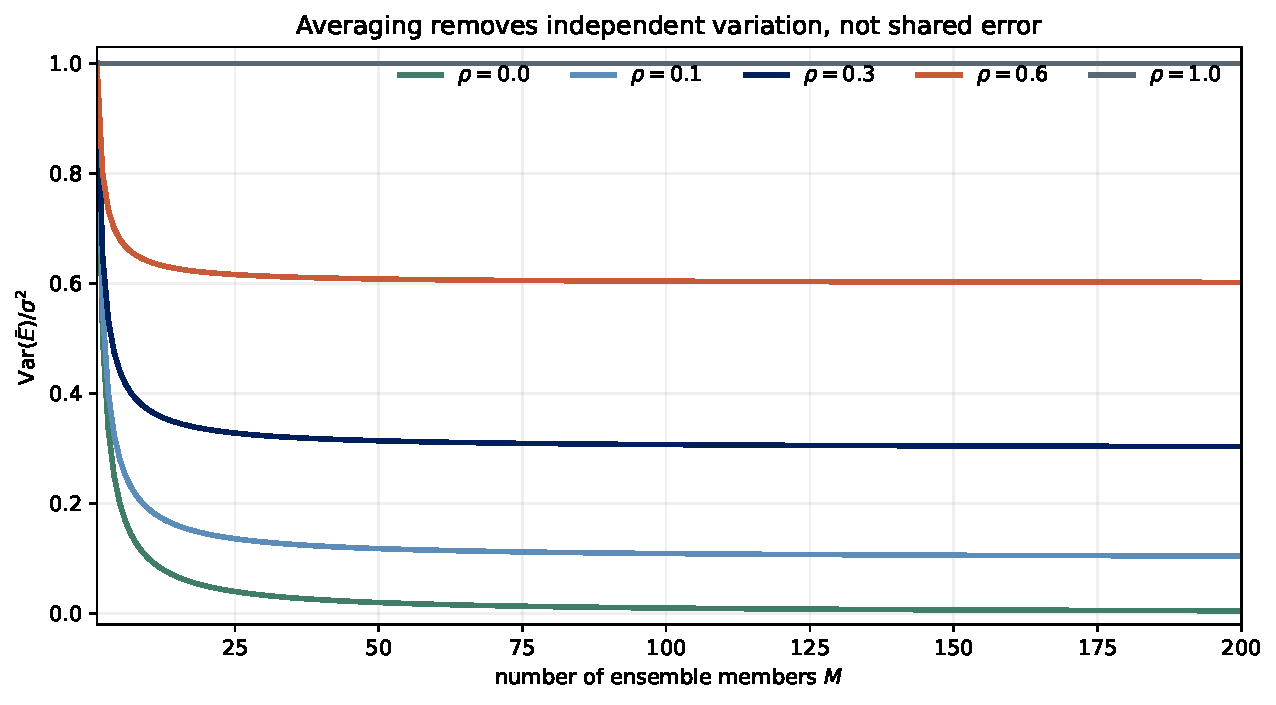
\includegraphics[width=0.88\textwidth]{figures/generated/ensemble-correlation-variance.pdf}
  \caption{Relative variance of an equally weighted ensemble under the
  equal-correlation model. Member count suppresses independent variation but
  cannot remove error shared by all members.}
  \label{fig:ensemble-correlation}
\end{figure}

The theorem is a model, not a guarantee. Real members can have different
variances, correlations, and biases. Averaging primarily targets variance; it
does not automatically remove shared bias or data leakage.

\begin{misconceptionbox}
\textbf{Misconception:} any diverse collection improves prediction.
\textbf{Correction:} deliberately bad members can be diverse and still damage
an ensemble. Diversity is useful only together with competence, and the gain
must survive held-out evaluation under the intended dependence structure.
\end{misconceptionbox}

\conceptcheck{Two ensembles contain equally accurate members. The first has
pairwise error correlation $0.15$ and the second $0.80$. Under the theorem's
assumptions, which has the lower limiting variance as $M\to\infty$, and what
does that say about adding more nearly identical members?}

\section{Bootstrap sampling and bagging}

Given observations indexed by $1,\dots,n$, a bootstrap sample draws $n$
indices independently and uniformly \emph{with replacement}. Repeated and
omitted observations are expected. For any row $i$,
\[
  \Pr(i\text{ is omitted})=\left(1-\frac1n\right)^n
  \longrightarrow e^{-1}\approx0.368.
\]
Thus a large bootstrap sample contains approximately $63.2\%$, or
$1-e^{-1}\approx0.632$, of the distinct training observations.

Bagging fits a base learner $F_m$ to each bootstrap sample and aggregates.
For regression,
\[
  \widehat F_{\mathrm{bag}}(x)=\frac1M\sum_{m=1}^{M}F_m(x).
\]
For classification, members may vote on labels or, preferably when available,
average aligned class probabilities. Deep trees are natural members because
they are competent and unstable: bootstrap perturbation produces meaningfully
different partitions, while averaging suppresses some of that variation.

The bootstrap creates no new scientific information. It approximates repeated
sampling from the empirical distribution and perturbs the fitted algorithm.
If rows are clustered by patient, site, instrument, or time, ordinary row
bootstrap sampling may destroy the dependence structure. The resampling unit
must match the population and deployment question.

\subsection{Out-of-bag evidence}

Observation $i$ is \emph{out of bag} for member $m$ when the $m$th bootstrap
sample omitted it. An OOB prediction for $i$ aggregates only members that did
not train on $i$:
\[
  \widehat F_{\mathrm{OOB}}(x_i)
  =\frac{1}{|\mathcal M_i|}\sum_{m\in\mathcal M_i}F_m(x_i),
  \qquad
  \mathcal M_i=\{m:i\text{ is OOB for }m\}.
\]
This provides economical internal evidence for debugging and rough selection.
It does not replace a final audit, repair grouped or temporal leakage, or
simulate a future population shift.

\begin{workedexample}{why an unstable tree can benefit from bagging}
Suppose two nearly tied root splits exist. A few changed rows make a single
tree choose one or the other, producing large downstream differences. Across
bootstrap samples both structures appear. If their held-out errors are not
perfectly aligned, probability averaging can be more stable than either
structure. A shallow, highly constrained tree may vary less and therefore gain
less from bagging. The observation ``bagging helps unstable learners'' follows
from a mechanism that can be measured, not from a model-name rule.
\end{workedexample}

\section{Random forests: decorrelate the trees}

A random forest adds feature randomization to bootstrap aggregation. At each
split, a tree considers only a random subset of the $p$ predictors. A common
classification default is roughly $\sqrt p$ candidate features, but the value
is a hyperparameter, not a law.

If one strong predictor is available to every split, many bagged trees may ask
the same root question and remain highly correlated. Feature subsampling forces
some trees to discover alternative predictive structure. This can weaken an
individual tree while improving the average by reducing member-error
correlation. Figure~\ref{fig:forest-mechanism} separates row perturbation,
feature perturbation, and aggregation.

\begin{figure}[htbp]
  \centering
  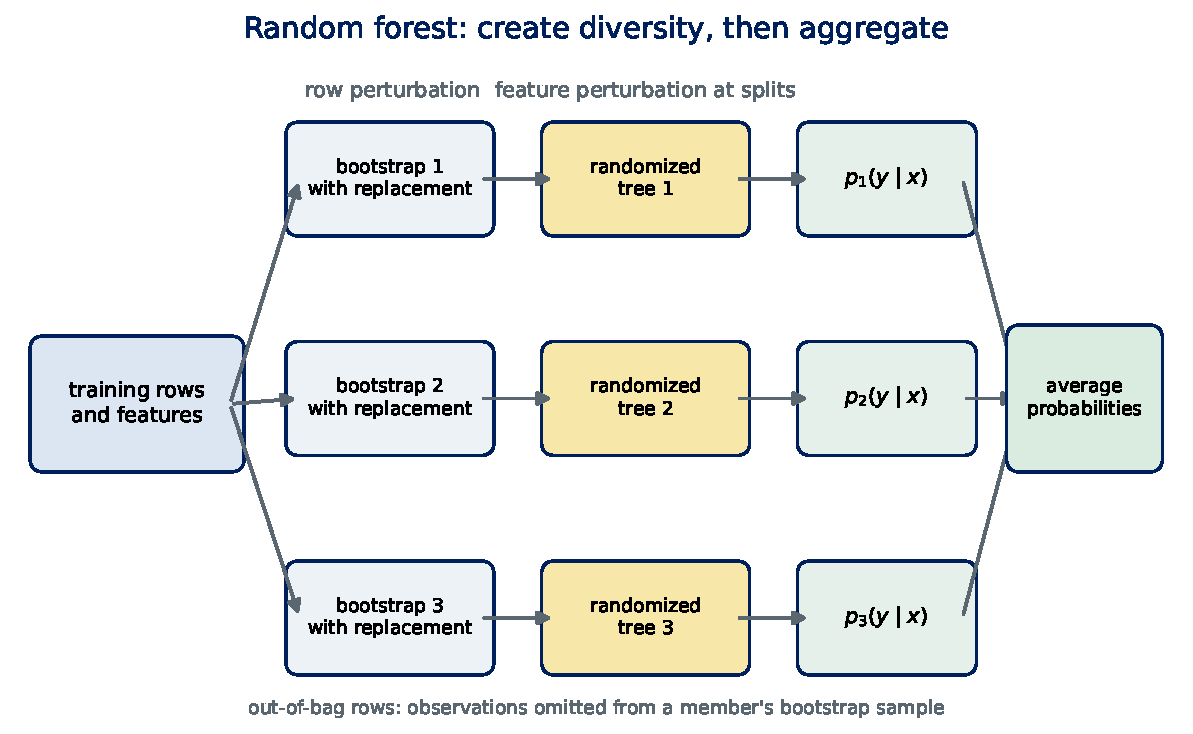
\includegraphics[width=0.96\textwidth]{figures/generated/random-forest-mechanism.pdf}
  \caption{A random forest draws bootstrap rows, grows trees with random
  candidate features at their splits, and averages aligned class
  probabilities. Rows omitted from a member's draw support OOB evidence.}
  \label{fig:forest-mechanism}
\end{figure}

Extremely randomized trees, or extra trees, inject additional randomness into
candidate thresholds and may use the full sample rather than bootstrap rows.
They can reduce correlation and computation while increasing bias. The proper
question is not which name sounds most advanced, but how bias, variance,
stability, probability quality, and resource cost change under a frozen
evaluation design.

More trees usually stabilize a forest average rather than overfit in the same
way as increasing single-tree depth. Nevertheless, depth, leaf size, feature
sampling, class weighting, bootstrap policy, and threshold choice still change
the learned function. Member count also increases fit cost, artifact size,
memory, and inference work.

\subsection{Probability aggregation is an interface contract}

For classes $\mathcal C=(c_1,\dots,c_K)$, let member $m$ return
$p_{mk}(x)$. The forest probability is
\[
  \overline p_k(x)=\frac1M\sum_{m=1}^{M}p_{mk}(x).
\]
Every vector must use the same class order. A bootstrap member may observe no
examples of a rare class; implementation code must insert a zero column in the
correct location rather than silently shifting columns. Tests should assert
shape, class order, finite values, range, and row sums.

The class decision $\arg\max_k\overline p_k(x)$ is separate from probability
quality. For a binary task, ROC AUC evaluates ranking; log loss and Brier score
evaluate probabilities; a decision threshold encodes consequences. A forest
can rank well and still be poorly calibrated.

\subsection{Feature importance does not identify scientific mechanism}

Mean decrease in impurity accumulates split improvements attributed to each
feature. It is fast but can favor variables with many candidate thresholds and
divide credit unpredictably among correlated predictors. Permutation importance
measures held-out degradation after shuffling a feature under a specified
perturbation. Correlated substitutes can conceal one another, and unrealistic
permutations can leave the data manifold. Neither method turns association into
causation.

Interpretation should therefore be scoped: ``this fitted artifact relied on
this feature under this perturbation and evaluation distribution.'' Stability
across folds, seeds, batches, and plausible perturbations is useful evidence.

\section{Boosting builds an additive model sequentially}

Bagging members can be fitted independently. Boosting constructs a sequence:
\[
  F_M(x)=F_0(x)+\sum_{m=1}^{M}\nu h_m(x),
\]
where $h_m$ is usually a shallow tree and $0<\nu\le1$ is a learning rate or
\emph{shrinkage}. Each stage depends on the current model. Parallelizing this
dependency is fundamentally different from parallelizing a forest.

For empirical risk
\[
  \mathcal R(F)=\frac1n\sum_{i=1}^{n}L(y_i,F(x_i)),
\]
define the negative gradient at stage $m$ by
\[
  r_{im}=-\left.
  \frac{\partial L(y_i,f)}{\partial f}
  \right|_{f=F_{m-1}(x_i)}.
\]
The base learner is fitted so that $h_m(x_i)\approx r_{im}$, and the model
updates to $F_m=F_{m-1}+\nu h_m$. This is gradient descent in a space of
functions, restricted to directions representable by the base learner.

\begin{theorem}[squared-error boosting fits residuals]
For half squared-error loss
$L(y,f)=\tfrac12(y-f)^2$, the negative gradient with respect to the prediction
$f$ is the residual $y-f$.
\end{theorem}

\begin{proof}
Differentiation gives
\[
  \frac{\partial}{\partial f}\frac12(y-f)^2=f-y.
\]
Negating this derivative gives $y-f$. Evaluating at
$f=F_{m-1}(x_i)$ yields
$r_{im}=y_i-F_{m-1}(x_i)$.
\end{proof}

The best constant initializer for squared error is the training-target mean.
The first tree fits residuals from that mean; the next fits residuals from the
updated additive model. Figure~\ref{fig:boosting-sequence} depicts successive
corrections.

\begin{figure}[htbp]
  \centering
  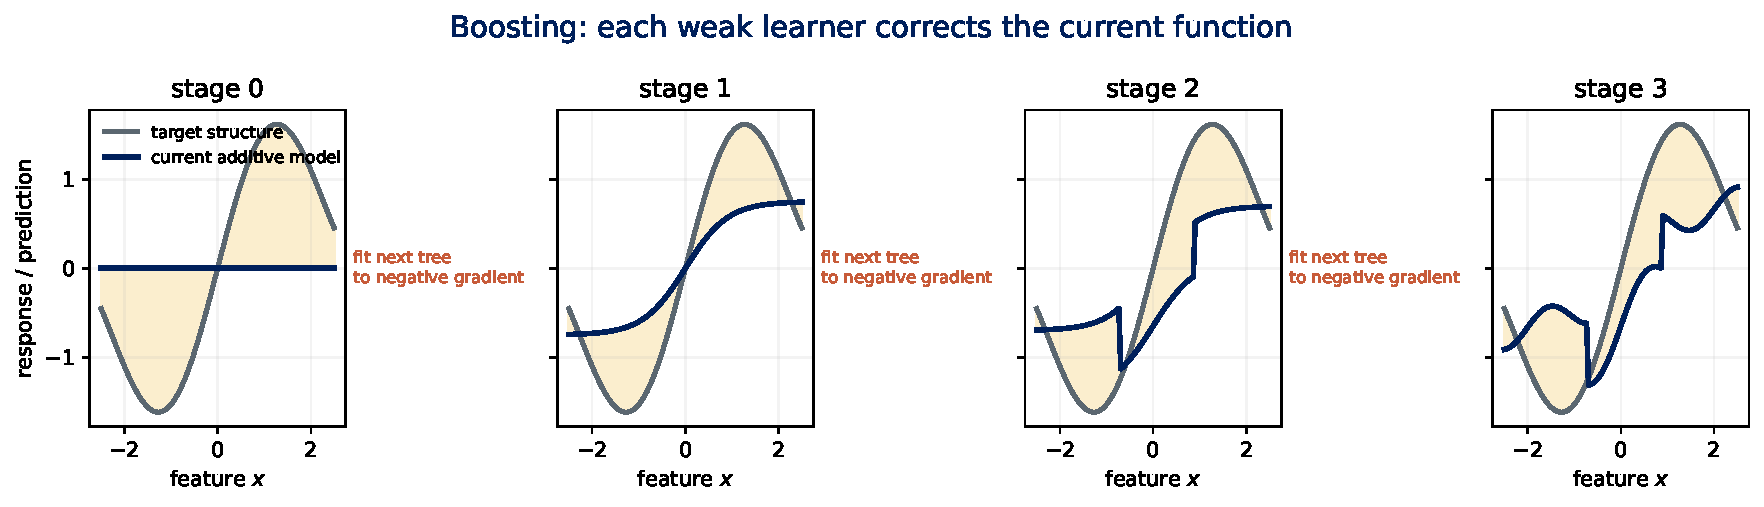
\includegraphics[width=0.98\textwidth]{figures/generated/boosting-stagewise-correction.pdf}
  \caption{A boosted model begins with a simple function and adds restricted
  learners toward current negative gradients. The shaded discrepancy changes
  after every stage.}
  \label{fig:boosting-sequence}
\end{figure}

\subsection{Classification gradients}

For a binary logit $F$, probability $p=\sigma(F)$, and cross-entropy
\[
  L(y,F)=\log(1+e^F)-yF,
\]
the derivative is $p-y$, so the negative gradient is $y-p$. Each new learner
approximates a correction related to probability residuals. Numerical
implementations also optimize leaf values and apply regularization; the phrase
``fit residuals'' must always be interpreted relative to the chosen loss.

AdaBoost follows a related but distinct route. With labels and weak predictions
in $\{-1,+1\}$, weighted error is
\[
  \epsilon_m=\sum_i w_i\mathbf 1\{y_i\ne h_m(x_i)\}.
\]
When $\epsilon_m<1/2$, define
\[
  \alpha_m=\frac12\log\frac{1-\epsilon_m}{\epsilon_m},
  \qquad
  w_i\leftarrow
  \frac{w_i\exp(-\alpha_m y_i h_m(x_i))}{Z_m}.
\]
Misclassified observations gain relative weight. The final score is a weighted
vote. Hard or mislabeled observations can consequently receive increasing
attention, making data auditing essential.

\subsection{Shrinkage, depth, and stopping}

Learning rate and stage count interact. Small $\nu$ takes conservative steps
and generally requires more stages. It is not free regularization: additional
stages increase fit time, prediction time, and artifact size. Tree depth
controls the interaction order available in one correction. Stumps represent
main effects; deeper trees represent higher-order interactions but can chase
noise more readily.

Early stopping monitors a validation trace and halts after improvement ceases.
The monitoring data must remain inside the training boundary. If final test
data determine the stopping stage, they are no longer an honest final audit.
Nested selection may be required when comparing many losses, depths, learning
rates, and stage budgets.

Histogram-based implementations bin feature values to accelerate split search.
XGBoost, LightGBM, CatBoost, and scikit-learn's histogram estimators differ in
category handling, missing-value routing, regularization, distributed or GPU
execution, determinism, and serialization. A library is a versioned dependency
with a behavioral contract, not merely an import.

\begin{workedexample}{a regression booster as an auditable sequence}
Begin with $F_0=\overline y$. Store the stage-one residuals, fitted tree, and
updated predictions. Repeat while recording training and validation loss after
each stage. A behavior test uses a hand-computable piecewise-constant target and
verifies the initializer, staged prediction count, and decreasing training
loss. A production comparison then checks a trusted histogram booster on the
same split. This separates mechanism verification from optimized implementation
evaluation.
\end{workedexample}

\conceptcheck{Why can adding more trees to a random forest and adding more
stages to a boosted ensemble have different overfitting behavior? Identify the
parallel averaging mechanism in the first and the adaptive optimization path in
the second.}

\section{Leakage-safe out-of-fold stacking and voting}

Hard voting returns the modal class label and discards confidence. Soft voting
averages class probabilities, optionally with validation-selected weights.
Soft voting requires aligned class orders and probabilities whose calibration
is sufficiently comparable. A confidently wrong member can dominate an
unweighted mean.

Stacking learns a meta-model from base-model outputs. The tempting procedure
fits each base learner on all training rows, predicts those same rows, and fits
the meta-model on the resulting predictions. Those in-sample predictions are
optimistically biased: the meta-model learns from information unavailable at
future inference.

Correct stacking constructs out-of-fold (OOF) features. Partition training rows
into folds. For each fold, fit base models on the remaining folds and predict
the reserved fold. Every training row's meta-features then come from base models
that did not train on that row. Refit base models on all training data only
after the meta-model has been trained. Figure~\ref{fig:stacking-boundary}
contrasts the two data flows.

\begin{figure}[htbp]
  \centering
  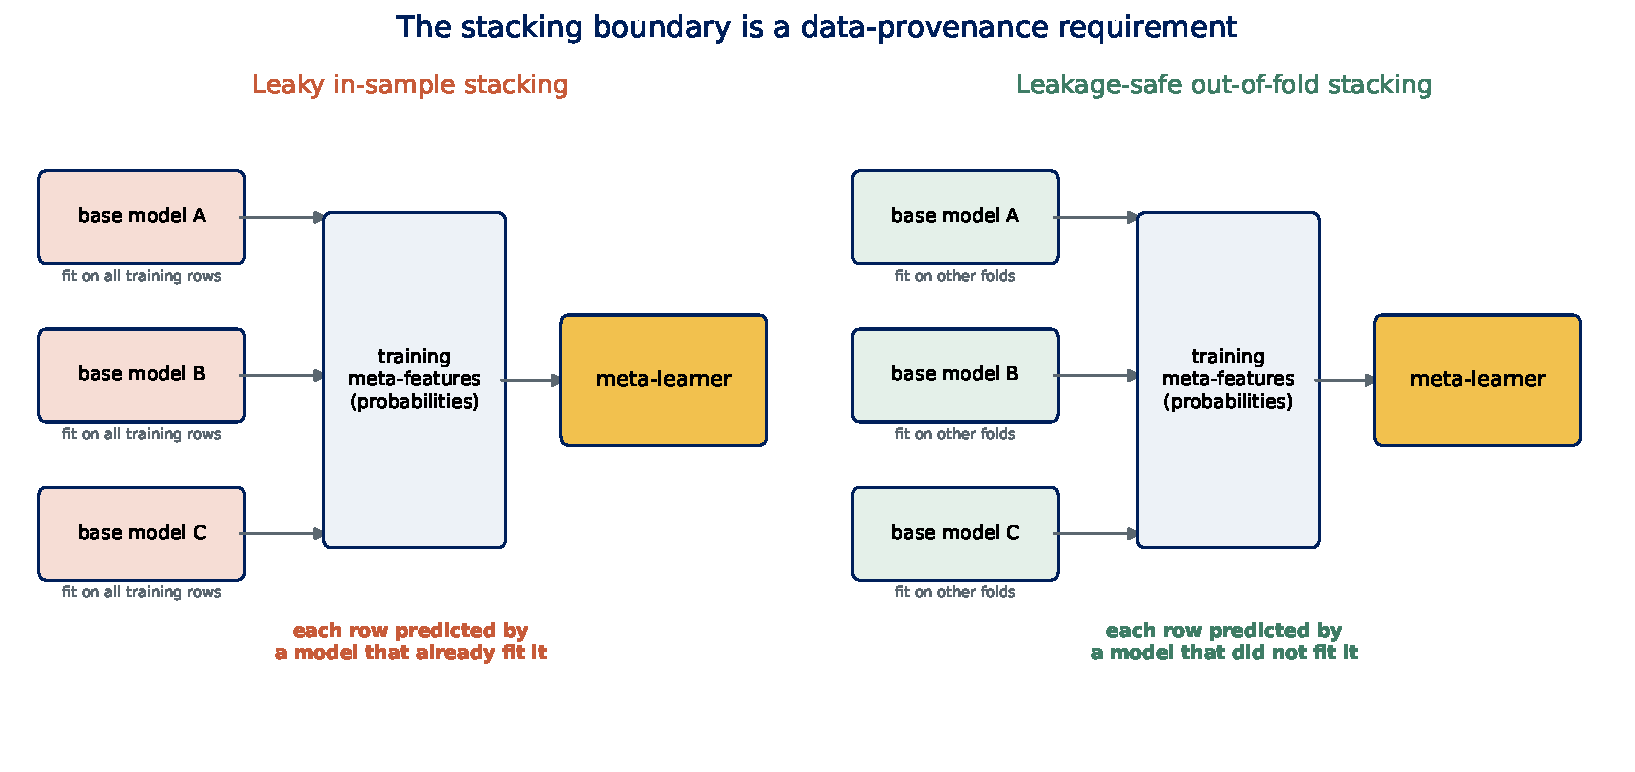
\includegraphics[width=0.98\textwidth]{figures/generated/stacking-oof-boundary.pdf}
  \caption{In-sample base predictions leak fitted-row performance into the
  meta-model. Out-of-fold construction preserves a training-row information
  boundary: each row is predicted by a base model that did not fit it.}
  \label{fig:stacking-boundary}
\end{figure}

If there are $B$ base learners and $K$ classes, raw probability meta-features
have $BK$ columns. Every block should be finite, lie in $[0,1]$, sum to one,
and follow a tested class order. Preprocessing must be fitted inside every base
fold. The folds must also preserve groups, time, or other dependence from the
original problem.

\begin{warningbox}
Out-of-fold does not automatically mean leakage-safe. Shuffled row folds remain
wrong when multiple rows describe the same patient, when future observations
predict the past, or when preprocessing was fitted globally. The stacking split
must inherit the original information and dependence boundaries at every level.
\end{warningbox}

\section{Evaluation is a systems comparison}

An ensemble may improve one predictive metric while harming probability
quality, class-specific performance, latency, memory, energy, portability, or
maintainability. Compare candidates under a common evidence contract:

\begin{center}
\begin{tabularx}{0.95\textwidth}{@{}lX@{}}
\toprule
Evidence family & Questions \\
\midrule
Predictive & Which loss and metrics match the decision? What is uncertainty in
the difference? \\
Probability & Are probabilities calibrated overall and where decisions are
made? Are class orders and thresholds correct? \\
Stability & Do conclusions survive seeds, folds, batches, subgroups, and
plausible perturbations? \\
Operational & What are fit cost, batch throughput, tail latency, memory,
serialized size, and energy where material? \\
Governance & Can the complete artifact be rebuilt, tested, owned, monitored,
rolled back, and explained at an appropriate scope? \\
\bottomrule
\end{tabularx}
\end{center}

The \emph{champion} is the approved artifact currently serving the contract. A
\emph{challenger} is evaluated under the same split, preprocessing, metrics,
calibration procedure, and resource budget. Promotion should require a
practically meaningful gain and no unacceptable regression, not merely the
largest point estimate among many trials.

\begin{workedexample}{forest and boosting challengers}
For future-batch degradation prediction, a calibrated logistic champion is
compared with a random forest and a histogram gradient booster. Hyperparameters
and early stopping use earlier batches only. The final batch is audited once.

The booster improves average precision but overstates event probability. A
calibrator is fitted without touching the final batch. The promotion report
compares decision cost, calibration, batch uncertainty, artifact size, and
prediction latency. Promotion is withheld when the gain disappears on the
newest batch. That is a successful evaluation: it prevented unjustified system
complexity.
\end{workedexample}

\section{Software engineering contracts for ensembles}

Reusable code belongs in a module, not duplicated across notebooks. An
inspectable forest should expose fitted members, bootstrap indices, seeds, OOB
counts and probabilities, classes, feature count, and importances. An
inspectable booster should expose the initializer, ordered stage learners,
learning rate, staged predictions, and loss trace.

Tests should include:
\begin{itemize}
  \item hand-computable bootstrap and additive-update examples;
  \item deterministic reconstruction under a fixed seed;
  \item probability shape, range, class order, and row sums;
  \item OOB coverage and exclusion of in-bag predictions;
  \item initializer and staged-loss behavior for squared-error boosting;
  \item prediction-before-fit, dimensional mismatch, nonfinite data, and invalid
  hyperparameters;
  \item differential checks against a trusted library on unambiguous fixtures;
  \item serialization, schema, and supported-runtime smoke tests; and
  \item an explicit test that rejects leaky stacking features.
\end{itemize}

CI uses small lawful fixtures. Full student-supplied data belongs outside Git
when license, privacy, or size demands it; provenance, schema, checksum, and
retrieval instructions remain versioned. Applied notebooks import the package,
state a question, and present evidence. They are not a second implementation of
the algorithm.

\begin{misconceptionbox}
\textbf{Misconception:} the most accurate ensemble is the most professional
model. \textbf{Correction:} professional quality is conditional on the system
contract. A smaller calibrated model may be superior when the ensemble's point
gain is unstable, operationally expensive, difficult to monitor, or unsupported
in the deployment runtime.
\end{misconceptionbox}

\section{Exercises}
\begin{enumerate}
  \item Derive the equal-correlation variance theorem without assuming equal
  means. State why means do not enter the variance calculation.
  \item For $n=5$, compute the exact probability that a specified observation
  is OOB from a size-five bootstrap sample. Compare it with $e^{-1}$.
  \item Design an experiment that separates member competence from member-error
  correlation for bagging and random forests.
  \item Prove that the mean is the constant minimizing squared-error loss and
  connect this result to the gradient booster's initializer.
  \item Derive the negative gradient of binary cross-entropy written as
  $\log(1+e^F)-yF$.
  \item Explain why learning rate, stage count, and tree depth cannot be tuned
  independently of the validation design.
  \item Draw the data flow for five-fold stacking with three base learners and
  three classes. Label every fit and prediction boundary.
  \item Construct a test that fails for in-sample stacking features but passes
  for correct OOF features.
  \item Compare impurity and permutation importance under two strongly
  correlated predictors. Explain why disagreement need not be a bug.
  \item Write a champion--challenger gate covering predictive quality,
  calibration, class-specific regressions, artifact size, latency, and
  deterministic rebuild.
  \item In the companion student project, contribute one ensemble component
  with package code, analytic and failure tests, a lawful CI fixture, and a
  question-led notebook using student-supplied data. Your pull request must
  explain added operational cost and one reason not to promote the model.
\end{enumerate}

\begin{chapterreview}
Ensembles improve learning through structured diversity, not member count
alone. Bagging perturbs observations and averages unstable learners. Random
forests also randomize candidate features to lower member correlation; OOB
predictions provide useful internal evidence with important limits. Boosting
constructs an additive sequence guided by negative loss gradients; for squared
error, those gradients are residuals. Voting combines decisions or
probabilities, while stacking requires out-of-fold meta-features and tested
class alignment. Any predictive gain must survive probability, dependence,
stability, interpretation, software, and resource evidence before promotion.
\end{chapterreview}

\begin{notebooklink}
Lecture 15 notebook 00 derives bagging and random forests on the Wisconsin
Diagnostic Breast Cancer data. Lecture 15 notebook 01 derives residual and
gradient boosting on diabetes-progression data and compares production
estimators. Lecture 15 notebook 02 constructs leakage-safe voting and stacking
on UCI Wine data and closes with a champion--challenger promotion gate. Each
laboratory includes the exact companion-project code, test, data, and pull-
request boundary.
\end{notebooklink}
